\pagestyle{empty}
\chapter*{\centering \large DAFTAR RIWAYAT HIDUP}
\thispagestyle{empty}

\begin{wrapfigure}{l}{4cm}
	\vspace{-25pt}
	\begin{center}
		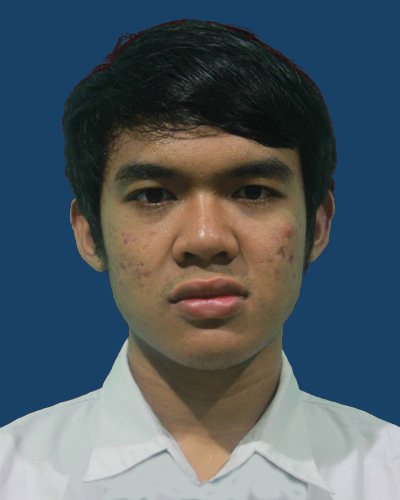
\includegraphics[width=0.27\textwidth]{gambar/pas-foto}
	\end{center}
	\vspace{-80pt}
\end{wrapfigure}

\noindent \textbf{GREGORIUS ANDITO HERJUNO.}  Lahir di Jakarta, 20 November 1994.  Anak kedua dari pasangan Bapak Mickael Sudadi dan Ibu Maria Adi Retno SK. Saat ini beralamatkan di Cluster Adena blok SA2 No. 7 Graha Raya Bintaro.

\vspace{0.5cm}
\noindent
\begin{center}
	\begin{flushright}
		\begin{tabular}{lcl}
			No. Ponsel	& :&  087881123212 \\
			Email	& :&  gregorius.andito@gmail.com
		\end{tabular}
	\end{flushright}
\end{center}
\vspace{0.5cm}

\noindent \textbf{Riwayat Pendidikan} : Penulis mengawali pendidikan di TKK Sang Timur Karang Tengah pada tahun 1999 - 2001, dan kemudian melanjutkan pendidikan di SDK Sang Timur Karang Tengah pada tahun 2001 - 2007. Setelah itu, penulis melanjutkan ke SMPK Sang Timur Karang Tengah hingga tahun 2010. Kemudian kembali melanjutkan ke SMA Santa Laurensia pada tahun 2010 dan melanjutkan ke SMA Candle Tree pada tahun 2011 - 2013. Di Tahun yang sama penulis melanjutkan ke Universitas Negeri Jakarta (UNJ), Program Studi Ilmu Komputer, melalui jalur UMBPTN. Di awal tahun 2017 (Kamis, 9 Februari 2017) penulis telah memperoleh gelar Sarjana Komputer (S.Kom), Program Studi Ilmu Komputer, Fakultas Matematika dan Ilmu Pengetahuan Alam, Universitas Negeri Jakarta.

\noindent \textbf{Riwayat Organisasi} : Selama di bangku perkuliahan, penulis aktif di organisasi keilmiahan Program Studi Ilmu Komputer sebagai anggota merangkap Wakil Ketua periode 2014-2015. Penulis juga berpartisipasi dalam kegiatan BINER (Be Innovative and Educated Researcher) yaitu kegiatan workshop dan seminar yang diadakan oleh DEFAULT, dimana penulis tergabung sebagai anggota merangkap Ketua Pelaksana. 

\noindent \textbf{Riwayat Penelitian} : Selain mengikuti organisasi, peneliti juga aktif dalam kegiatan Penelitian Dosen FMIPA UNJ bersama Dr. Makmuri, M.Si tahun 2015 dan 2016. 